
The control system of the autonomous x-wing fighter is shown in Fig.~\ref{fig:overview}. Overall, after a state estimator (Fig.~\ref{fig:overview}(h–i)) estimates the x-wing fighter's pose, a guidance system (Fig.~\ref{fig:overview}(g)) produces desired velocities, telling the direction toward waypoints. A controller (Fig.~\ref{fig:overview}(e–f)) then stabilizes and produces actuator commands sending to the x-wing fighter model (Fig.~\ref{fig:overview}(b–d)) to stabilize and move the fighter accordingly. Finally, the x-wing fighter is visualized in a simulation (Fig.~\ref{fig:overview}(a)). The github repository of this project is available at \textcolor{red}{xxxxxxxxxxxxxxxxxxxxxxxxx}.

\begin{figure*}[!htbp]
	\centering
	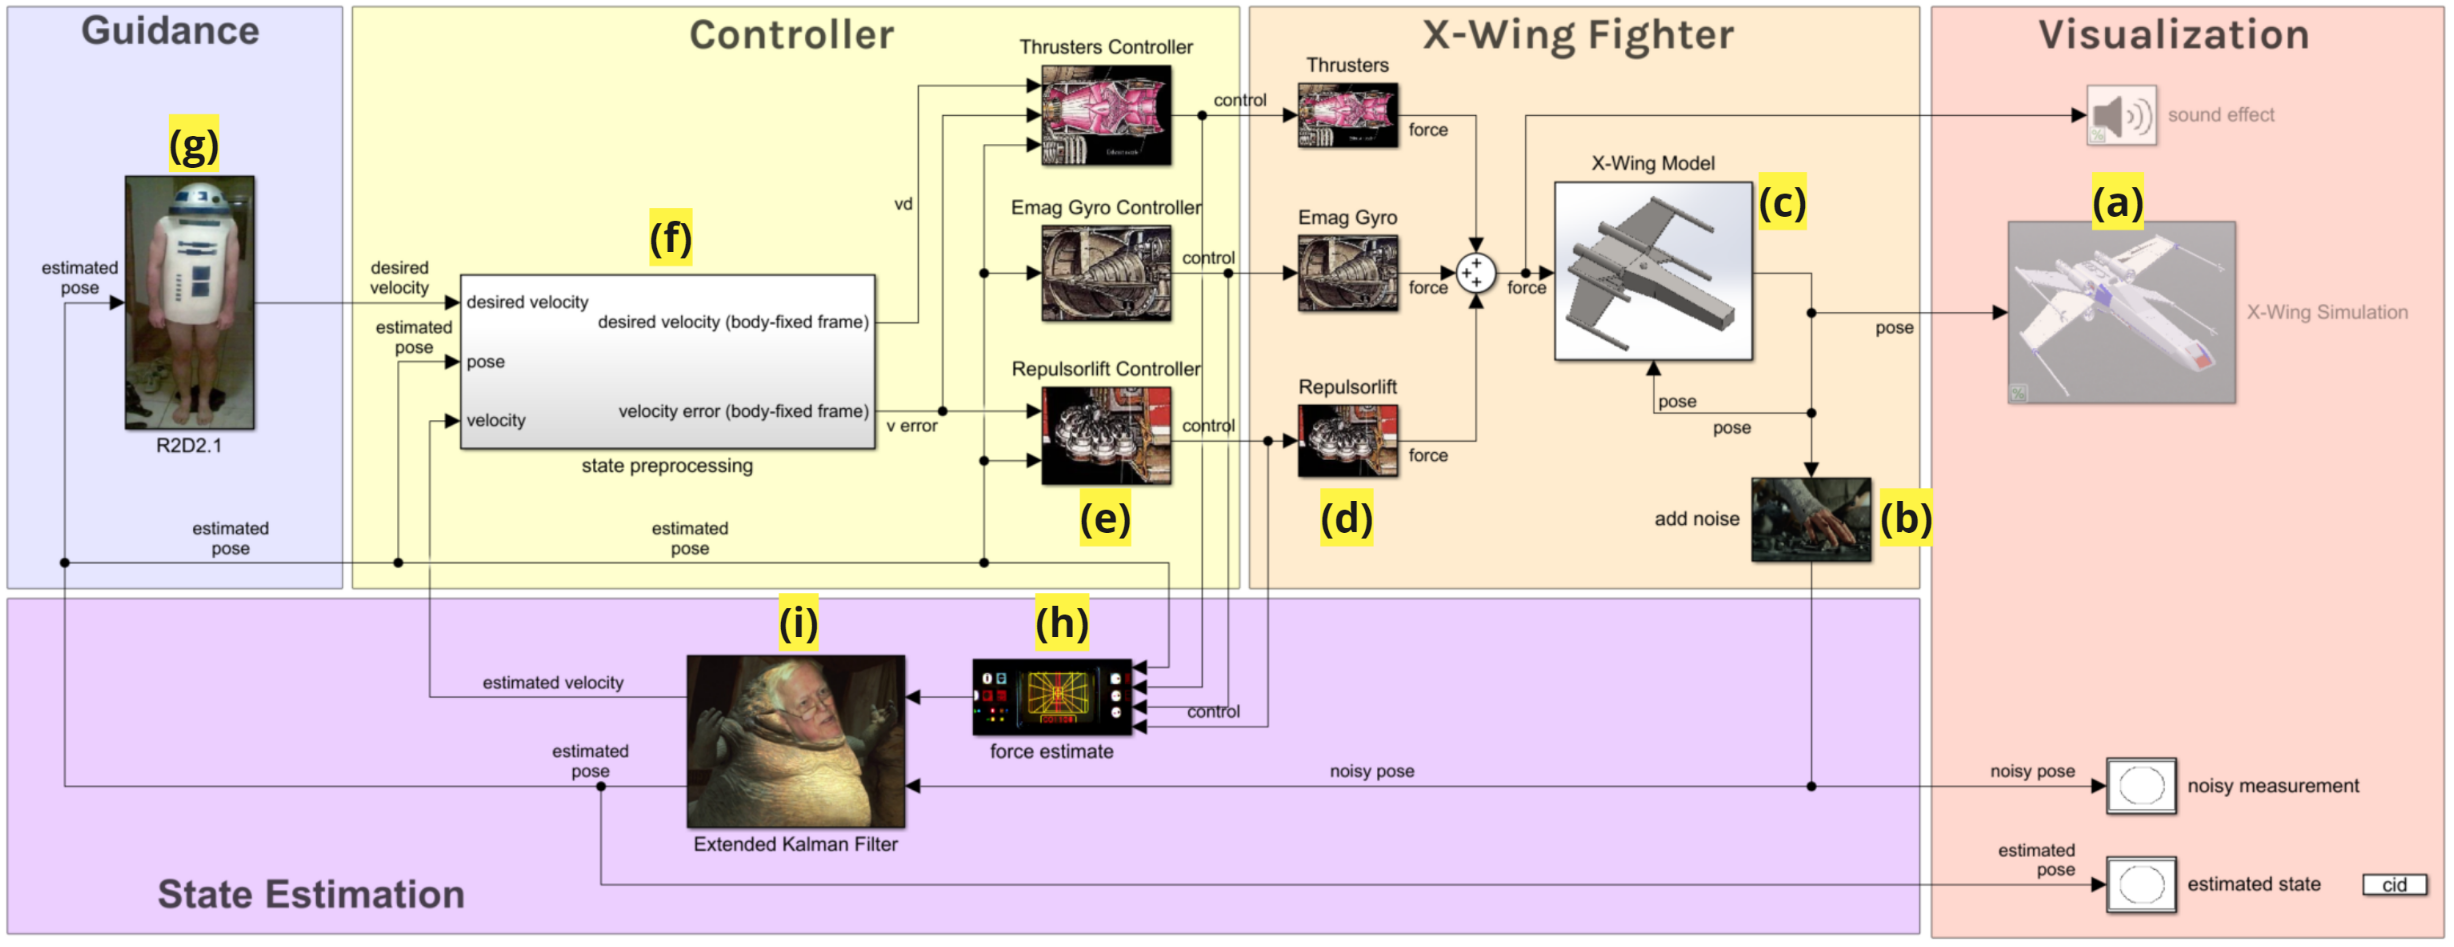
\includegraphics[width=0.85\linewidth]{figures/overview}
	\caption{Control system of the autonomous x-wing fighter, consisting of five key components: (a) simulation, (b–d) x-wing fighter model, (e–f) controller, (g) guidance system, and (h–i) state estimator.}
	\label{fig:overview}
\end{figure*}


